\documentclass[10pt,letterpaper,addpoints]{exam}
\usepackage[utf8]{inputenc}
\usepackage[spanish,es-noshorthands]{babel}
\usepackage{hyperref}
\usepackage{amsmath}
\usepackage{amsfonts}
\usepackage{amssymb}
\usepackage{graphicx}
\usepackage{tikz,pgf}
\usepackage{multicol}
\usepackage[width=7in,height=9.5in]{geometry}
%\printanswers
\begin{document}
\title{\begin{minipage}{.2\textwidth}
        
\includegraphics[height=1.75cm]{Images/logo-colegio.png}
       \end{minipage}
\begin{minipage}{.55\textwidth}
 \begin{center}
``Prueba sólidos''\\Geometría $9^{\circ}$
\end{center}
\end{minipage}
\begin{minipage}{.2\textwidth}

\includegraphics[height=1.75cm]{Images/logo-sed.png} 
\end{minipage}
}
\author{Germ\'{a}n Avendaño Ram\'{i}rez~\thanks{Lic. Matemáticas U.D., M.Sc. U.N.}}
\date{}
\maketitle
\begin{center}
\fbox{\fbox{\parbox{5.5in}{\centering
Conteste cada pregunta en el cuadro de respuestas. Debe hacer los procedimientos en su cuaderno}}}
\end{center}
\vspace{0.1in}
\makebox[\textwidth]{Nombres: \hrulefill, curso:\underline{\hspace{48pt}}, fecha:\underline{\hspace{3cm}}}
\begin{multicols}{2}
 \begin{questions}
 \question Observe la siguiente pirámide.
 \begin{center}
 \begin{tikzpicture}
 \draw (0,0,0)--(3,0,0)--(3.6,1,0)--(.6,1,0) --cycle;
 \draw (0,0,0)--(2.6,2.6,1.5)--(3,0,0);
 \draw (.6,1,0)--(2.6,2.6,1.5)--(3.6,1,0);	
 \end{tikzpicture}
 \end{center}
 ¿Con cuáles de los siguientes desarrollos planos se puede formar la pirámide?
 \begin{center}
 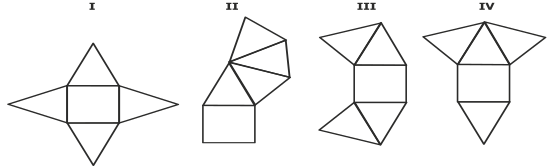
\includegraphics[scale=.45]{Images/Pantallazo.png} 
 \end{center}
 \begin{choices}
 \CorrectChoice Con I, II y IV solamente
 \choice Con II y con IV solamente
 \choice Con II, con III y con IV solamente
  \choice Con I y III solamente
 \end{choices}
 \question Observe la casa 
 \begin{center}
 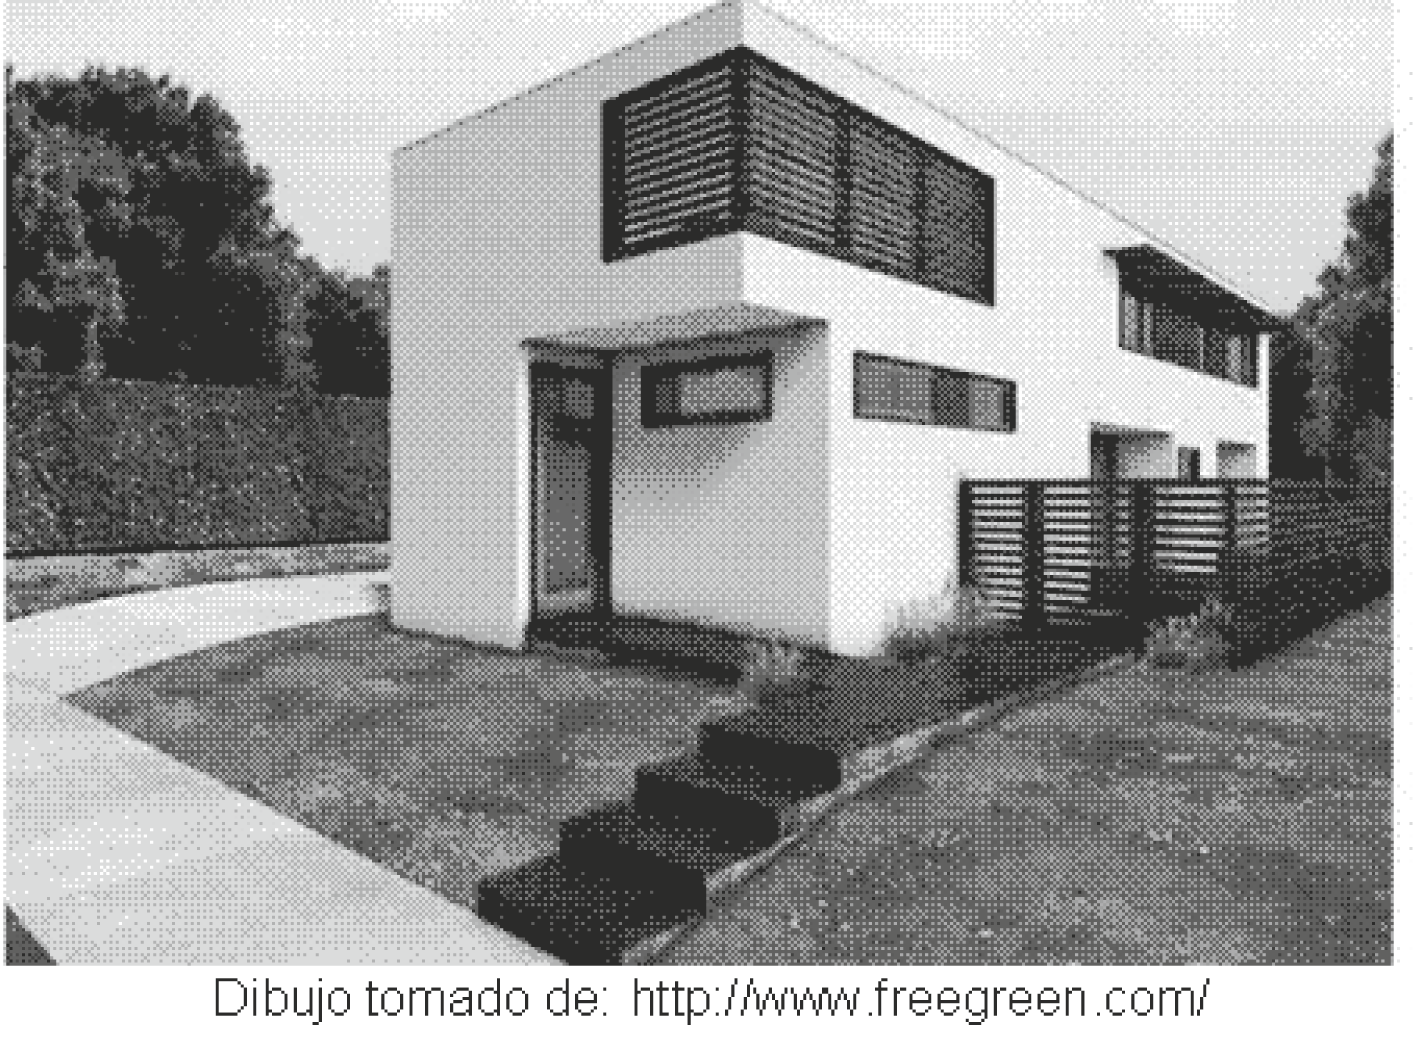
\includegraphics[scale=.15]{Images/frente-casa.png} 
 \end{center}
 ¿Cuál es la vista de frente de esta casa?
 \begin{center}
 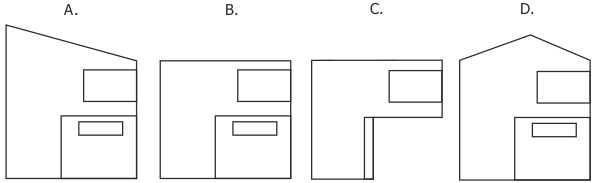
\includegraphics[scale=.45]{Images/Pantallazo-1.png} 
 \end{center}
 \question Un carpintero construye un mueble que tiene cajones como el que aparece en la siguiente figura:
 \begin{center}
 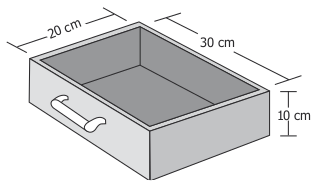
\includegraphics[scale=.6]{Images/Pantallazo-2.png} 
 \end{center}
 ¿Cuál es la capacidad en cm$^{3}$ de uno de los cajones del mueble?
 \begin{choices}
 \choice 500 cm$^{3}$
 \choice 4000 cm$^{3}$
 \CorrectChoice 6000 cm$^{3}$
  \choice 60 cm$^{3}$
 \end{choices}
 \question Con el molde que se presenta a continuación se va a construir un dado. A cada uno de los cuadrados en el molde, se le asignó uno de los números del 1 al 6 como se ilustra.
 \begin{center}
 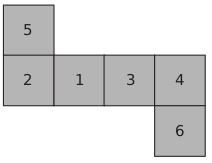
\includegraphics[scale=.6]{Images/Pantallazo-3.png} 
 \end{center}
 ¿En cuál de las siguientes figuras se muestra la ubicación correcta de los números en las caras del dado?
 \begin{center}
 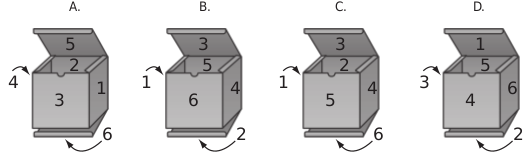
\includegraphics[scale=.45]{Images/Pantallazo-4.png} 
 \end{center}
 \question En un supermercado se empacan botellas de aceite del mismo tamaño en cajas rectangulares con capacidad para 6 botellas, como se muestra en la siguiente figura.
 \begin{center}
 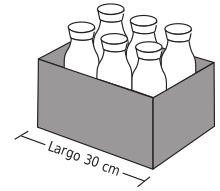
\includegraphics[scale=.6]{Images/Pantallazo-5.png} 
 \end{center}
 Una caja rectangular del mismo ancho que el de la figura, en la que se puedan empacar 8 de estas botellas, debe tener
 \begin{choices}
 \choice 35 cm de largo
 \CorrectChoice 40 cm de largo
 \choice 60 cm de largo
  \choice 33 cm de largo
 \end{choices}
 \question Las siguientes figuras representan dos tipos de recipientes, I y II, utilizados para empacar alimentos.
 \begin{center}
 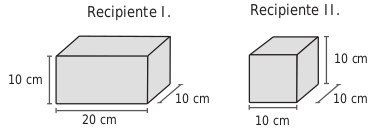
\includegraphics[scale=.6]{Images/Pantallazo-6.png} 
 \end{center}
 ¿Cuál de las siguientes afirmaciones, respecto al espacio ocupado por los recipientes tipo I y tipo II, es correcta?
 \begin{choices}
 \choice El recipiente tipo II ocupa el doble del espacio utilizado por el recipiente tipo I.
 \choice Cuatro recipientes tipo I ocupan el mismo espacio que tres recipientes tipo II.
 \choice Cuatro recipientes tipo II ocupan el mismo espacio que tres recipientes tipo I.
 \CorrectChoice El recipiente tipo I ocupa el doble del espacio utilizado por el recipiente tipo II.
 \end{choices}
 \question ¿Cuál de las figuras que se muestran a continuación, representa un sólido que tiene exactamente 6 caras?
 \begin{center}
 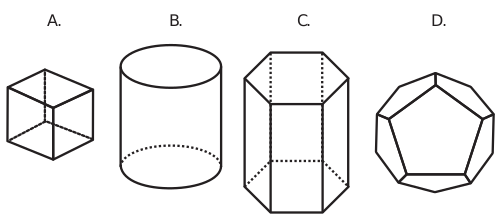
\includegraphics[scale=.45]{Images/Pantallazo-8.png} 
 \end{center}
 \question La siguiente figura representa un prisma triangular.
 \begin{center}
 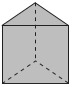
\includegraphics[scale=.75]{Images/Pantallazo-9.png} 
 \end{center}
 ¿Cuál(es) de los siguientes desarrollos planos permite(n) armar un prisma triangular?
 \begin{center}
 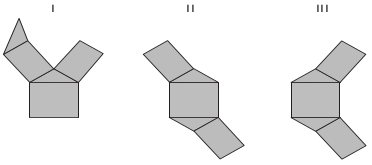
\includegraphics[scale=.65]{Images/Pantallazo-10.png} 
 \end{center}
 \begin{choices}
 \choice III solamente
 \CorrectChoice I y II solamente
 \choice I y III solamente
  \choice II solamente
 \end{choices}
 \end{questions}
\end{multicols}
\end{document}
